\sectionquestion{k-Nearest Neighbors}

\begin{parts}
\part You are given a training dataset containing information about various species of strawberries. Each species is described by its weight (in grams) and its sweetness (on a scale from 0 to 5). You want to use $k$-NN to classify which species are popular. You create a binary classification task by assigning a species a label of $+$ if the species is popular and $-$ otherwise. Consider the following dataset:
\begin{align*}
    D &= \{(x^{(i)}, y^{(i)})\}_{i=1}^{7}\\
    &= \{((1,4),+),((2,1),-),((2,4), +), ((3,2), -),((3,3),-),((4,1),+),((4,4),+)\}
\end{align*}
where $\xv^{(i)} \in \mathbb{R}^{2} = (\text{weight}, \text{sweetness})$ and $y^{(i)} \in \{+, -\}$ is the label.

For your convenience, we've plotted this dataset in the figure below:

\begin{center}
    \begin{tikzpicture}
        \begin{axis}[
            scale=1.5, axis equal image, mark options={scale=1.5},
            xmin=0, xmax=5, xtick={1,...,4},
            ymin=0, ymax=5, ytick={1,...,4},
            samples=50, grid=major, xlabel=Weight, ylabel=Sweetness]]
            \addplot [
                scatter,
                only marks,
                point meta=explicit symbolic,
                scatter/classes={
                    a={mark= +,blue},
                    b={mark= -,red}
                },
                nodes near coords*={$\xv^{(\pgfmathprintnumber[frac]\myvalue)}$},
                visualization depends on={\thisrow{myvalue} \as \myvalue},
            ] table [meta=label] {
                x y label myvalue
                1 4 a 1
                2 1 b 2
                2 4 a 3
                3 2 b 4
                3 3 b 5
                4 1 a 6
                4 4 a 7
            };
        \end{axis}
    \end{tikzpicture}   
\end{center}
        
You fit a $k$-NN model to this training dataset using the Euclidean distance. When computing the nearest neighbors, if two points are equally close to some input, ties are broken by selecting the less sweet species; if the two points are equally sweet, we break ties in favor of the less heavy species. % (Example tie scenario: if $k=2$, $(1,3)$ and $(3,3)$ have the same euclidean distance with $(2,3)$, then we choose $(1,3)$ as the closest point.)

\begin{subparts}
    \begin{comment}
    \subpart[2] \textbf{Drawing:} Given the training dataset shown above, plot each data point in the graph below by drawing its label, either a $+$ or a $-$, in the correct location:

    \begin{center}
        \begin{tikzpicture}
        \begin{axis}[
            scale=1.5, axis equal image, mark options={scale=1.5},
            xmin=0, xmax=6, xtick={1,...,5},
            ymin=0, ymax=6, ytick={1,...,5},
            samples=50, grid=major, xlabel= Weight, ylabel=Sweetness]]
        \end{axis}
        \end{tikzpicture} 
    \end{center}
    \end{comment}

    \subpart[4] \textbf{Drawing:} On the figure provided above, draw the decision boundary for a $1$-NN model.
    
    \begin{soln}
        \begin{center}
        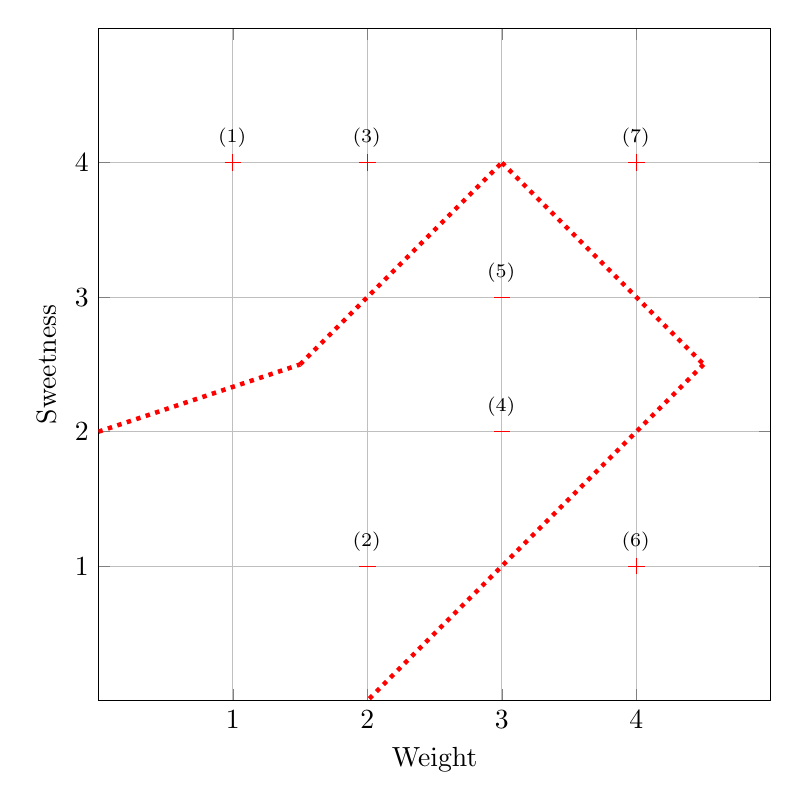
\begin{tikzpicture}
        \begin{axis}[
            scale=1.5, axis equal image, mark options={scale=1.5},
            xmin=0, xmax=5, xtick={1,...,4},
            ymin=0, ymax=5, ytick={1,...,4},
            samples=50, grid=major, xlabel=Weight, ylabel=Sweetness]]
            \addplot[red, ultra thick, dotted] coordinates { (0, 2) (1.5, 2.5) };
            \addplot[red, ultra thick, dotted] coordinates { (1.5, 2.5) (3, 4) };
            \addplot[red, ultra thick, dotted] coordinates { (3, 4) (4.5, 2.5) };
            \addplot[red, ultra thick, dotted] coordinates { (4.5, 2.5) (2, 0)};
            \addplot [
                scatter,
                only marks,
                point meta=explicit symbolic,
                scatter/classes={
                    a={mark= +,red},
                    b={mark= -,red}
                },
                nodes near coords*={$\xv^{(\pgfmathprintnumber[frac]\myvalue)}$},
                visualization depends on={\thisrow{myvalue} \as \myvalue},
            ] table [meta=label] {
                x y label myvalue
                1 4 a 1
                2 1 b 2
                2 4 a 3
                3 2 b 4
                3 3 b 5
                4 1 a 6
                4 4 a 7
            };
        \end{axis}
        \end{tikzpicture}   
        \end{center}
    \end{soln}
    \begin{qauthor}
        Zoe Xu, Describe a dataset as points in a high dimensional space
    
        Edited by Henry
    \end{qauthor}
    
    \subpart[2] \textbf{Numerical answer:} What is the training error of a $3$-NN on this dataset? \textbf{Report your answer as a fraction.}
    \begin{tcolorbox}[fit,height=1cm, width=2cm, blank, borderline={1pt}{-2pt}]
    %solution
    \end{tcolorbox}
    \begin{soln}
        $\frac{1}{7}$; I believe the only incorrectly predicted data point is $x^{(6)}$
    \end{soln}
    \begin{qauthor}
        Zoe Xu, implement $k$-NN algorithm and deal with tie scenario.

        Edited by Henry 
    \end{qauthor}

\begin{qtester}
    Should this be 3/7? x1, x7, x6?
    
    Zoe: Yes! Thank you very much. I should look at the answer more carefully.
\end{qtester}
    
    \subpart[2] \textbf{Select all that apply:} Let's say we have a new species with weight 1 and sweetness 3, and the new species is \textbf{not} popular among the market. For which values of $k$ is this new species correctly classified by a $k$-NN classifier?
    {
    \checkboxchar{$\Box$} \checkedchar{$\blacksquare$} % change checkbox style locally
    \begin{checkboxes}
     \choice $k = 1$
     \choice $k = 3$
     \choice $k = 5$
     \choice $k = 7$
     \choice None of the above
    \end{checkboxes}
    }
    \begin{soln}
    $C$
    \end{soln}
    \begin{qauthor}
        Zoe Xu, implement $k$-NN algorithm and deal with tie scenario.

        Edited by Henry
    \end{qauthor}
    \begin{qtester}
    At this point we are testing, so k=1 should not be valid right? 

    Zoe Xu: Yes! You're right. Thanks again!s
    \end{qtester}

    \subpart[2] \textbf{Short answer:} Looking at the training errors for different values of $k$, you choose the model with $k = 1$ as it has the lowest training error. Do you think this approach will lead to good performance on a held-out test dataset? If you answered yes, briefly justify your answer and if you answered no, briefly describe an alternative method that you think would lead to better performance; limit your response to 1-2 concise sentences. 
    
    \fillwithlines{9em}
    \begin{soln}
    No, we would use validation dataset (validation error) to choose k as k is a hyperparameter.
    \end{soln}
    \begin{qauthor}
        Zoe Xu (citing from practice problem Exam1 F23), one point for true or false, and one point for reason.
        Describe the inductive bias of a $k$-NN classifier
    \end{qauthor}

\end{subparts}

\part[2] \textbf{Select all that apply:} Which of the following statement(s) about $k$-NNs is/are true? % Assume a point can be its own neighbor.
    {%
    \checkboxchar{$\Box$} \checkedchar{$\blacksquare$} % change checkbox style locally
    \begin{checkboxes}
     \choice $k$-NN can be applied to classification problems but not regression problems.
     \choice We can always achieve zero training error with a $1$-NN model, but it may not generalize well in testing.
     \choice Decreasing $k$ can help address overfitting.
     \choice Computing the predictions of a $k$-NN model becomes more computationally expensive as the number of features grows. 
     \choice None of the above
    \end{checkboxes}
    }
    \begin{soln}
    $B, D$
    \end{soln}
    \begin{qauthor}
        Zoe Xu, test understanding of $k$-NN model
    \end{qauthor}

\clearpage

    \part[2] \textbf{Short Answer:} Suppose we have a binary classification task where the labels are coded as $y\in \{-1,+1\}$. We create the following variant of the $k$-NN classifer with $k=4$ that uses the Euclidean distance metric: $h(\xv') = \hat{y}' = \textrm{sign}(2y_1 + y_2 + y_3 + y_4)$, where $y_i$ is the label of the $i$-th closest point to $\xv'$ ($i = 1, 2, \cdots, 4$). Assume that there are at least $4$ data points in the training dataset. 
    
    Essentially, our model assigns double the weight to the closest point relative to the three other nearest neighbors. If there is a tie for the closest point to $\xv'$, then we choose an arbitrary point to get double the vote. Your friend claims that ties in the vote will never happen (i.e, the value inside the sign expression will never be $0$). Is your friend correct? Briefly justify your answer in 2-3 concise sentences. 
    \fillwithlines{15em}
    \begin{soln}
    Your friend is correct. Since each point is classified as +1 or -1, with three points, the only possible values for the sum are $\{-5, -4, -3, -1, 1, 3, 4, 5\}$. The value for the closest point is either +2 or -2, which means that if we add the values of all the points with the weights, we will never get 0.
    \end{soln}
    \begin{qauthor}
    Bhargav, Invent "new" k-NN learning algorithms capable of dealing with even k
    \end{qauthor}

\part[2] Suppose you train a $k$-NN classifier using Euclidean distance on \emph{binary} vectors $\x$ of length $D$, i.e., the value of each feature is either $0$ or $1$. Unfortunately, you find that the performance of your classifier on some held out test dataset $\mathcal{D}_{\textrm{test}}$ isn't very good. 

\textbf{True or False:} Switching from the Euclidean distance to the Manhattan distance \emph{could} improve the performance of your classifier on $\mathcal{D}_{\textrm{test}}$. Briefly justify your answer in 1-2 concise sentences. Recall that the Manhattan distance between vectors is: 
    
    \[d(\x,\x') = \sum_{i=1}^D |x_i-x_i'|\]
    
    \begin{checkboxes}
        \choice True
        \choice False
    \end{checkboxes}
    \fillwithlines{9em}
    \begin{soln}
        False; the Euclidean distance and Manhattan distance will behave identically on binary vectors in terms of determining relative distances between points. 
    \end{soln}

\end{parts}